\documentclass[11pt, a4paper]{article}

% Packages for Visual Presentation and Typography
\usepackage[utf8]{inputenc}
\usepackage{geometry}
\geometry{margin=1in}
\usepackage{graphicx}
\graphicspath{{images/}}
\usepackage{booktabs}
\usepackage{xcolor}
\usepackage{titlesec}
\usepackage{caption}
\usepackage{fancyhdr}
\usepackage{float}
\usepackage{microtype} % Dramatically improves text justification and readability
\usepackage{setspace} % Allows for cleaner line spacing
\onehalfspacing % Makes the document much easier to read

% Add these lines to set up APA formatting and link your .bib file
\usepackage[american]{babel} 
\usepackage{csquotes}
\usepackage[style=apa, backend=biber]{biblatex}
\addbibresource{references.bib} 

% Make sure this hyperref stuff stays BELOW the biblatex commands above
\usepackage{hyperref}
\hypersetup{
    colorlinks=true,
    linkcolor=blue!70!black,
    urlcolor=blue!70!black,
    citecolor=blue!70!black
}

\let\cleardoublepage\clearpage
\setlength{\headheight}{40pt}

% Title formats
\titleformat{\section}{\Large\bfseries\color{blue!70!black}}{\thesection}{1em}{}[\titlerule]
\titleformat{\subsection}{\large\bfseries}{\thesubsection}{1em}{}

% Header & Footer
\pagestyle{fancy}
\fancyhf{}
\fancyhead[L]{AI Pre-screening for Cardiac Murmurs}
\fancyhead[R]{Module 4 Project UNAM}
\fancyfoot[C]{\thepage}

% Title Page Information
\title{\textbf{Pre-screening of Heart Murmurs Using Artificial Intelligence}\\ \Large Multi-Modal Deep Learning for the Detection of Malignant Murmurs in Pediatric and Adult Populations}
\author{Javier Roberto Uribe Sandoval}
\date{\today}

\begin{document}

\maketitle
\thispagestyle{empty}

\newpage
\pagestyle{fancy}
\fancyhf{}
\fancyhead[L]{Universidad Nacional Autónoma de México}
% Ensure you have this logo in your directory, or comment this line out
\fancyhead[R]{
\includegraphics[height=1.5cm]{LOGO-UNAM-269x300.png}}
\fancyfoot[C]{\thepage}
\pagenumbering{arabic}

\tableofcontents

\newpage

% --- Section 1: Introduction ---
\section{Abstract \& Introduction}
Cardiovascular diseases remain a leading cause of mortality globally. The early detection of heart murmurs often precedes the diagnosis of structural or valvular defects, making it a critical screening step, especially in pediatric populations. However, the traditional use of a stethoscope for auscultation is highly subjective and susceptible to human error. Studies show that the diagnostic accuracy of primary care physicians using stethoscope auscultation alone can be surprisingly low, often ranging between 40\% and 70\% depending on the specific pathology \cite{davidsen2023diagnostic}.

To address this critical gap, this project develops a Deep Learning pre-screening tool utilizing the PhysioNet CirCor dataset \cite{reyna2022heart}. The objective is to engineer a highly sensitive, multi-modal artificial intelligence system capable of identifying acoustic anomalies. This system acts as a first-line filter, reliably flagging patients who require referral to a cardiologist for exhaustive echocardiographic review. 

% --- Section 2: Problem Statement ---
\section{Problem Statement}
The core problem addressed is the high rate of misdiagnosis and missed referrals in primary cardiac care due to the limitations of human auditory perception and subjective interpretation. Stethoscope auscultation relies heavily on the physician's experience, ambient noise levels, and the intermittent nature of murmurs. 

A computational approach is required to standardize this screening process. The solution must not only accurately classify complex, noisy audio signals but also account for the patient's physiological context (age, weight, height), as a benign acoustic pattern in a neonate may indicate a severe pathology in a young adult.

% --- Section 3: Strategy & Implementation ---
\section{Strategy and Implementation}
The core strategy of this project is to bridge the gap between primary care and specialized cardiology by providing an objective, AI-driven second opinion.

\subsection{Target Users and Needs}
The primary target users for this model are \textbf{General Practitioners (GPs), Pediatricians, and primary care nurses} operating in first-contact clinics. 
\begin{itemize}
    \item \textbf{Their Need:} These professionals are tasked with identifying subtle cardiac anomalies but often lack the specialized acoustic training or access to expensive echocardiogram equipment found in cardiology wards. 
    \item \textbf{The Solution:} They require a fast, objective tool that reduces the uncertainty of stethoscope auscultation in noisy clinic environments. The goal is not to replace the doctor, but to reduce "false negatives" (sending a sick child home) and "false positives" (over-referring healthy patients to expensive specialists).
\end{itemize}

\subsection{Model Usability}
For an AI model to be useful in a medical setting, it must be frictionless. To ensure high usability, the model is wrapped in a \textbf{Streamlit web dashboard} designed specifically for non-technical medical staff.
\begin{itemize}
    \item \textbf{Intuitive Interface:} The physician only needs to input basic demographic data (Age, Sex, Height, Weight) via simple dropdowns and sliders, and upload the digital stethoscope audio files (\texttt{.wav}). No coding or machine learning knowledge is required.
    \item \textbf{Explainability:} Instead of a "black box" prediction, the dashboard displays the exact Continuous Wavelet Transform (CWT) spectrogram that triggered the anomaly, allowing the doctor to visually see the murmur.
    \item \textbf{Clinical Integration:} The app features a one-click "Download PDF Report" button, instantly generating a formal, formatted document that can be directly attached to the patient's Electronic Health Record (EHR).
\end{itemize}

\subsection{Actionable Outcomes}
The predictions generated by the model trigger immediate, concrete clinical actions:
\begin{enumerate}
    \item \textbf{Triage and Referral:} If the model flags an anomaly and crosses the optimized confidence threshold, the immediate actionable is to issue a formal referral for a pediatric or adult cardiologist for an echocardiogram.
    \item \textbf{Patient Communication:} Physicians can use the generated PDF and visual spectrograms as an educational tool to transparently explain to the patient (or their parents) exactly why a specialist referral is necessary, increasing patient compliance.
    \item \textbf{Resource Optimization:} If the model confidently predicts a normal heart sound, the physician can comfortably discharge the patient, saving the healthcare system the cost of an unnecessary specialist consultation.
\end{enumerate}

% --- Section 4: Data Description & EDA ---
\section{Data Description and Exploratory Analysis}
\subsection{Data Source and Relevance}
The project utilizes the PhysioNet CirCor Cardiac Murmur dataset, a comprehensive collection of phonocardiogram (PCG) recordings paired with clinical metadata \cite{reyna2022heart}. The data is highly relevant as it represents real-world, noisy clinical environments rather than sterile laboratory conditions, ensuring the model learns robust, deployable features.
The dataset was last updated in May 2022 \cite{physionet2022}.

\subsection{Exploratory Data Analysis (EDA)}
An exhaustive exploratory analysis revealed several critical factors guiding the modeling strategy:
\begin{itemize}
    \item \textbf{Class Distribution:} The dataset exhibits a relatively balanced patient-level distribution (in the validation data set, there are approximately 91 Normal and 98 Abnormal patients), mitigating the need for aggressive synthetic oversampling techniques.
    \item \textbf{Variable Audio Lengths:} Audio recordings varied significantly in duration (from a few seconds to over a minute), necessitating a standardized windowing approach.
    \item \textbf{Clinical Correlations:} Analysis of the metadata indicated that murmurs are highly localized. A patient might exhibit a loud murmur at the Mitral Valve (MV) while the Aortic Valve (AV) sounds completely normal. This biological reality directly influenced the patient-level aggregation strategy used during evaluation.
\end{itemize}

\begin{figure}[htbp]
    \centering
    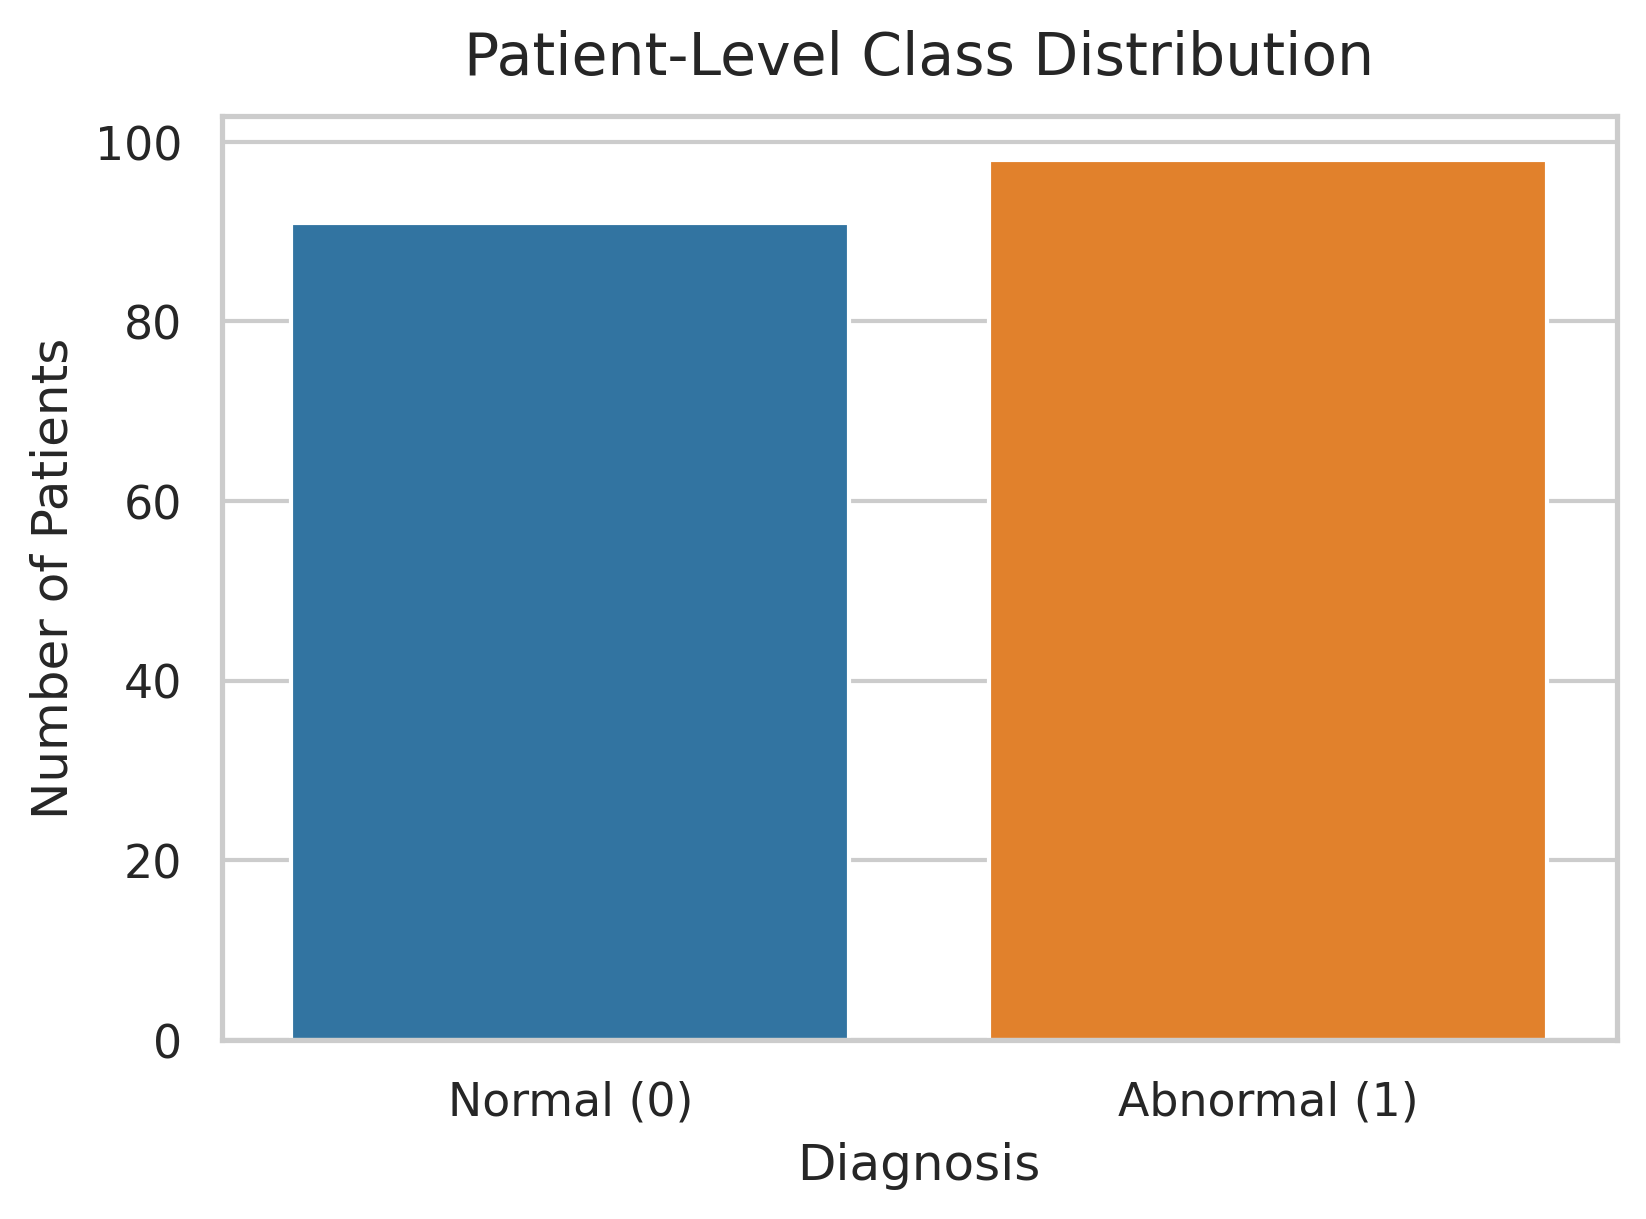
\includegraphics[width=0.6\textwidth]{class_distribution.png}
    \caption{Distribution of Normal vs Abnormal patient classes in the dataset.}
\end{figure}

% --- Section 5: Data Processing ---
\section{Data Processing and Engineering}
Raw medical audio is inherently noisy and cannot be fed directly into standard neural networks effectively. The following transformations were systematically applied and justified:

\begin{enumerate}
    \item \textbf{Fixed-Length Windowing:} To solve the variable length issue, audio files were algorithmically sliced into fixed 3.0-second overlapping windows. This standardization is mandatory for batch processing in Convolutional Neural Networks (CNNs).
    \item \textbf{Time-Frequency Transformation (CWT):} 1D soundwaves were converted into 2D Continuous Wavelet Transform (CWT) spectrograms. Unlike standard Fourier transforms, CWT maintains high resolution across both time and frequency domains, allowing the network to "see" the exact structural shape of the murmur.
    \item \textbf{Data Leakage Prevention:} Slicing audio explodes the dataset size. To prevent identical patient data from appearing in both training and testing sets, a \texttt{GroupShuffleSplit} was implemented based on the Patient ID.
    \item \textbf{Clinical Scaling:} Numerical metadata (Height, Weight) was normalized using a Min-Max Scaler. Crucially, the scaler was fitted solely on the training data and saved as an external object to transform inference data, ensuring mathematical consistency in deployment.
\end{enumerate}

\begin{figure}[htbp]
    \centering
    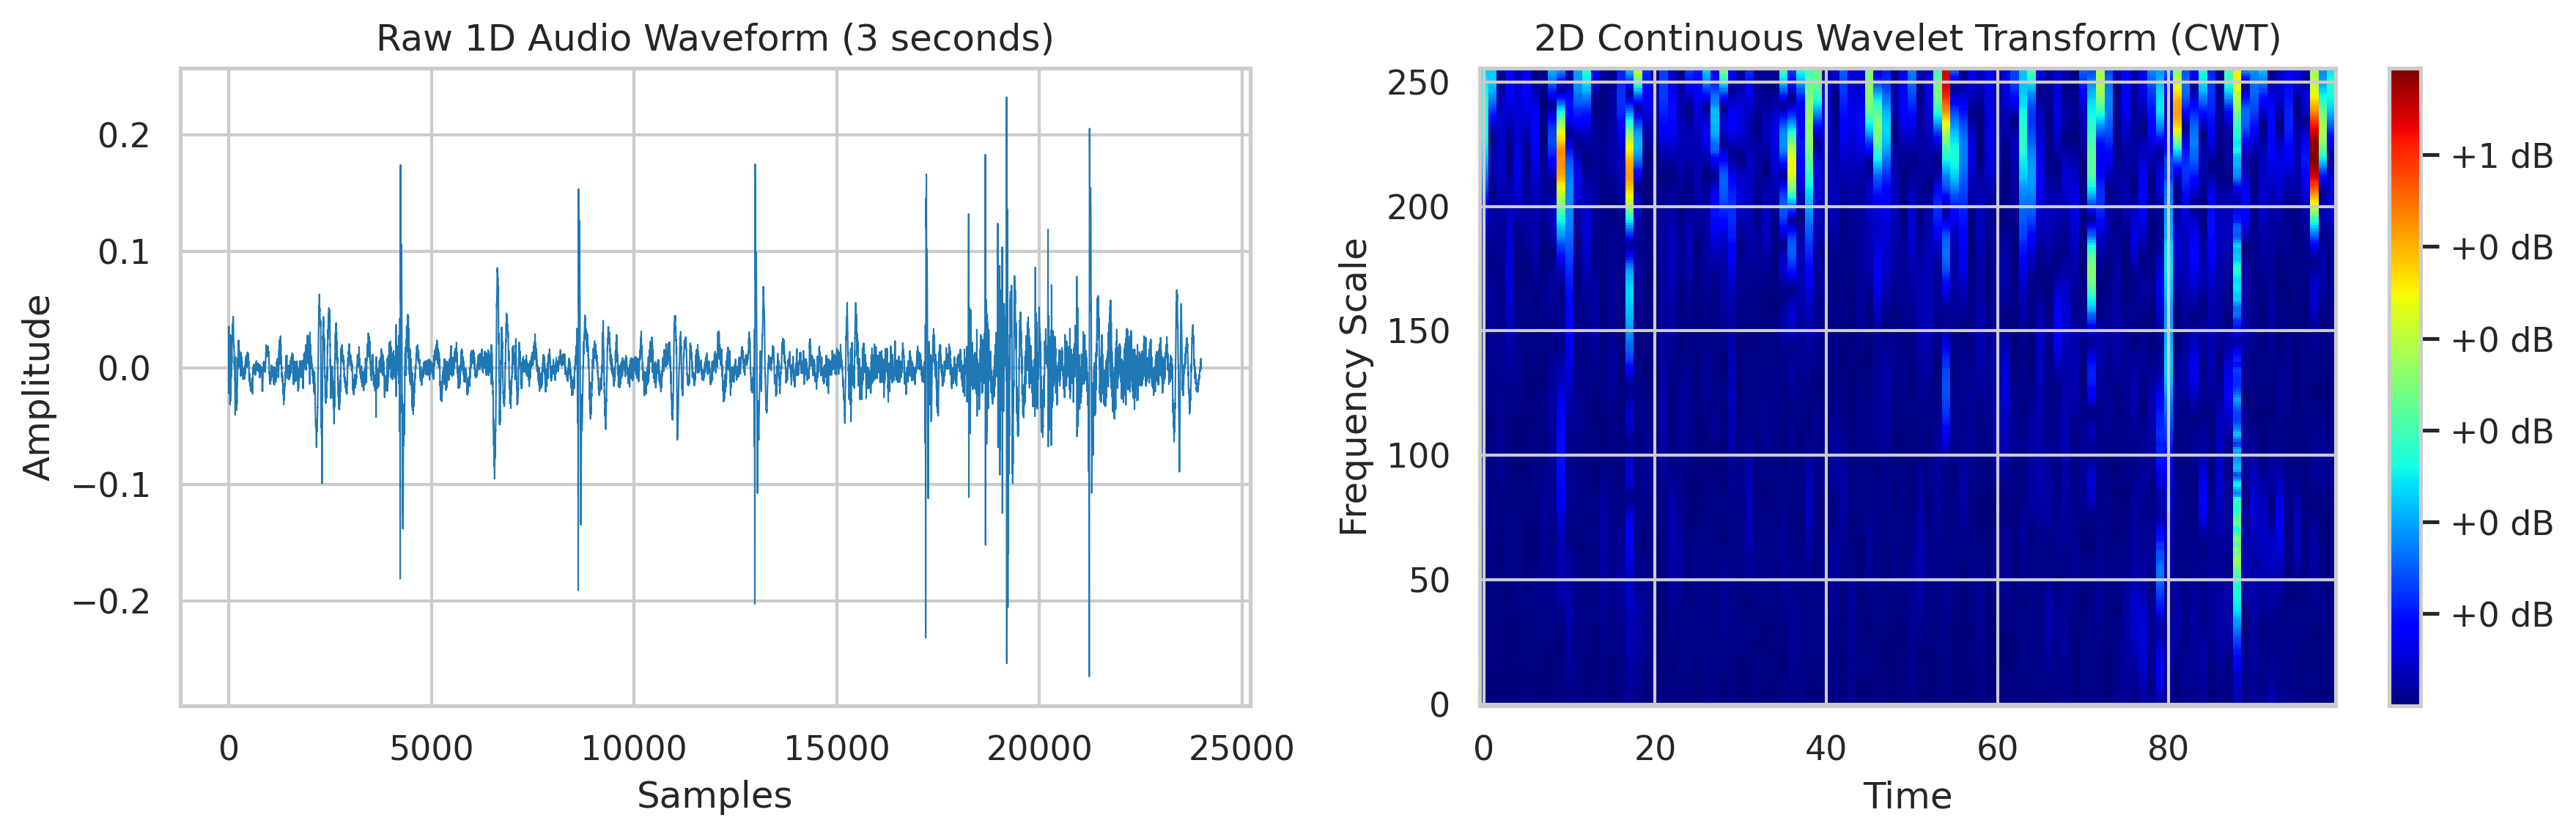
\includegraphics[width=0.8\textwidth]{cwt_transformation.png}
    \caption{Transformation of the 1D raw waveform into a 2D CWT spectrogram.}
\end{figure}

This dataset is predominantly based on children, but also includes neonates, infants, and a small subset of young adults (such as pregnant women).

\begin{figure}[htbp]
    \centering
    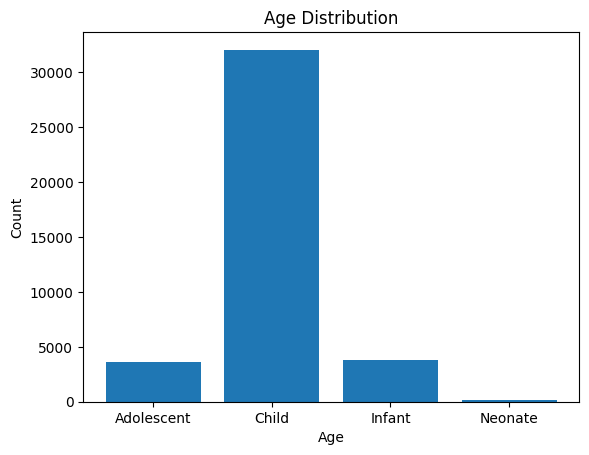
\includegraphics[width=0.8\textwidth]{age_distribution.png}
    \caption{The age group distribution of the participants in the dataset.}
\end{figure}

% --- Section 6: Strategy & Modeling ---
\section{Strategy and Multi-Modal Modeling}
The architecture developed goes beyond standard audio analysis by utilizing a Multi-Modal Fusion network.

\subsection{The Fusion Architecture}
Because heart sounds are dependent on physiology, the model splits into two processing streams:
\begin{itemize}
    \item \textbf{Audio Stream:} Processes the CWT spectrograms using deep CNNs acting as visual feature extractors.
    \item \textbf{Metadata Stream:} Processes encoded clinical variables (Age, Sex, Height, Weight, and Stethoscope Location) through dense neural layers.
\end{itemize}
These representations are concatenated before the final classification layers, granting the AI the necessary context to interpret the audio correctly.

\subsection{Model Selection and Fine-Tuning}
The following model was evaluated to maximize robust feature extraction:
\begin{itemize}
    \item \textbf{EfficientNetB0:} Highly sensitive to complex, high-frequency anomalies, utilizing compound scaling to maximize efficiency \cite{tan2019efficientnet}.
\end{itemize}
A two-phase fine-tuning strategy was employed: warming up the custom top layers, followed by unfreezing the entire base architecture with a micro-learning rate ($1e-5$). Furthermore, \textbf{Binary Focal Crossentropy} ($\gamma=2.0$) was utilized as the loss function \cite{lin2017focal}. This mathematically forces the network to dynamically scale gradients, focusing heavily on borderline, difficult-to-classify murmurs rather than easy predictions.

% --- Section 7: Resolution & Evaluation ---
\section{Problem Resolution and Performance Evaluation}
To mimic reality, model predictions were aggregated at the \textbf{Patient Level}. Instead of relying on a standard 0.5 threshold, an optimized threshold (T=0.56) was mathematically derived from the Receiver Operating Characteristic (ROC) curve to balance precision and recall.

\subsection{Performance Metrics}
The optimized model achieved a \textbf{Patient-Level AUC of 0.76}, demonstrating a strong, genuine ability to separate acoustic distributions. 

\begin{table}[htbp]
\centering
\caption{Optimized Patient-Level Classification Report (Threshold = 0.56)}
\begin{tabular}{lcccc}
\toprule
\textbf{Class} & \textbf{Precision} & \textbf{Recall (Sensitivity)} & \textbf{F1-Score} & \textbf{Support} \\
\midrule
Normal (0)  & 67.0\% & 70.0\% & 68.0\% & 91 \\
Abnormal (1)  & 71.0\% & 67.0\% & 69.0\% & 98 \\
\midrule
\textbf{Overall Accuracy} & \multicolumn{4}{c}{\textbf{68.8\%}} \\
\bottomrule
\end{tabular}
\end{table}

The metrics display a highly calibrated model. The balanced sensitivity and specificity ensure the system acts as a reliable filter without overwhelming cardiologists with false positives. This enables the first line doctors to effectively screen the majority of patients and reduce the workload for cardiologists.

\begin{figure}[htbp]
    \centering
    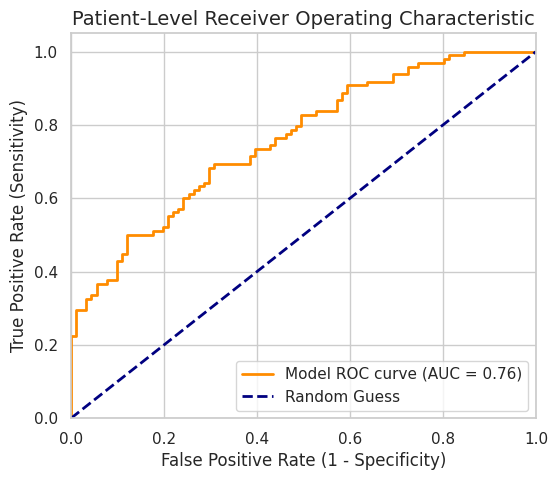
\includegraphics[width=0.45\textwidth]{roc_curve.png}
    \hfill
    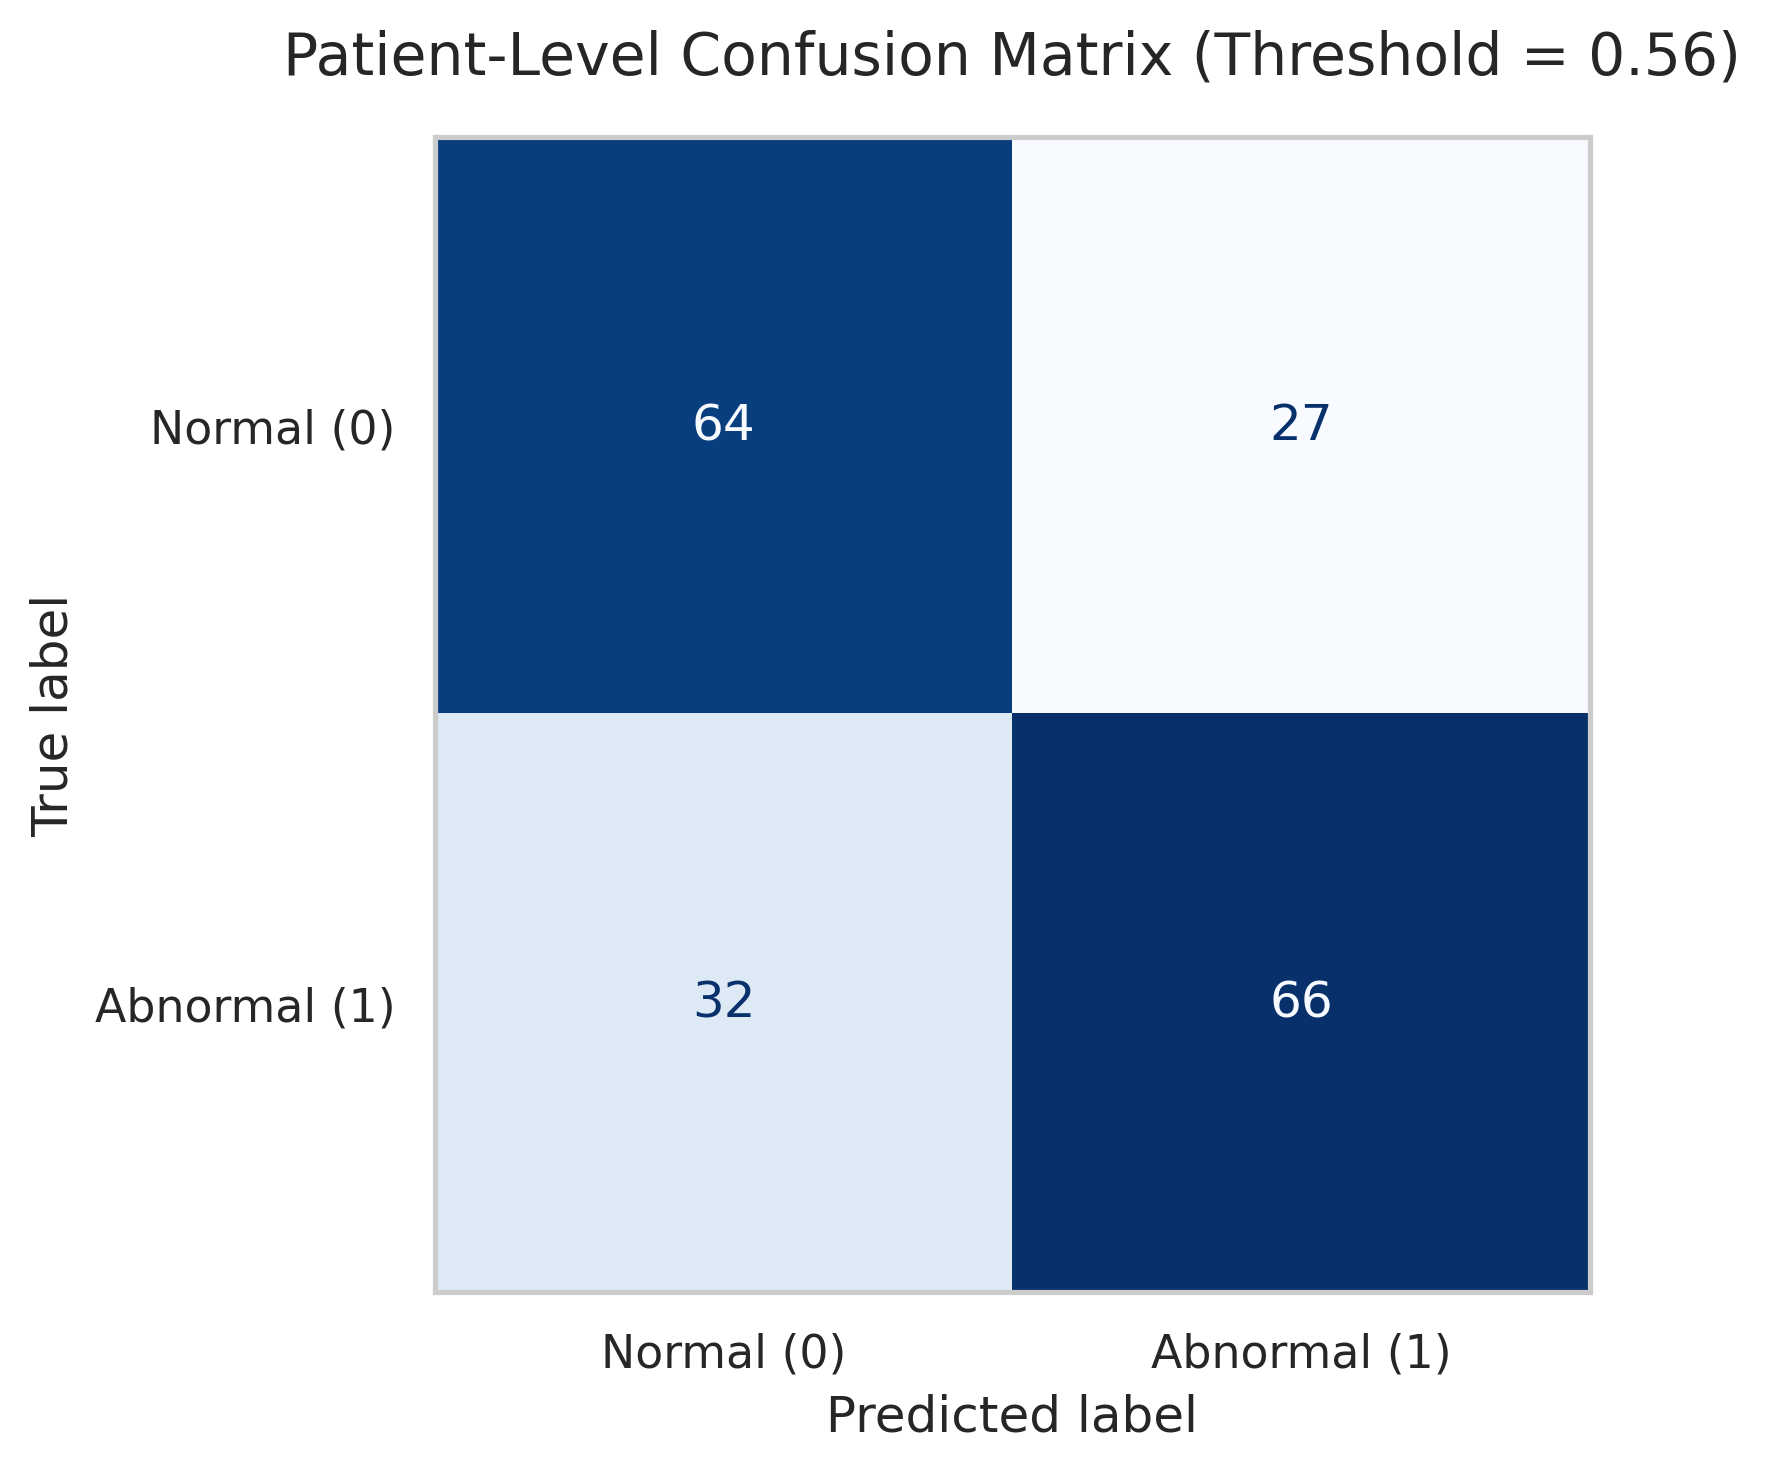
\includegraphics[width=0.45\textwidth]{confusion_matrix.png}
    \caption{Left: ROC Curve demonstrating AUC of 0.76. Right: Patient-Level Confusion Matrix.}
\end{figure}

\subsection{Deployment and Clinical Integration}
To truly resolve the problem, the model was packaged into an interactive clinical dashboard using \texttt{Streamlit}. 

\begin{figure}[htbp]
    \centering
    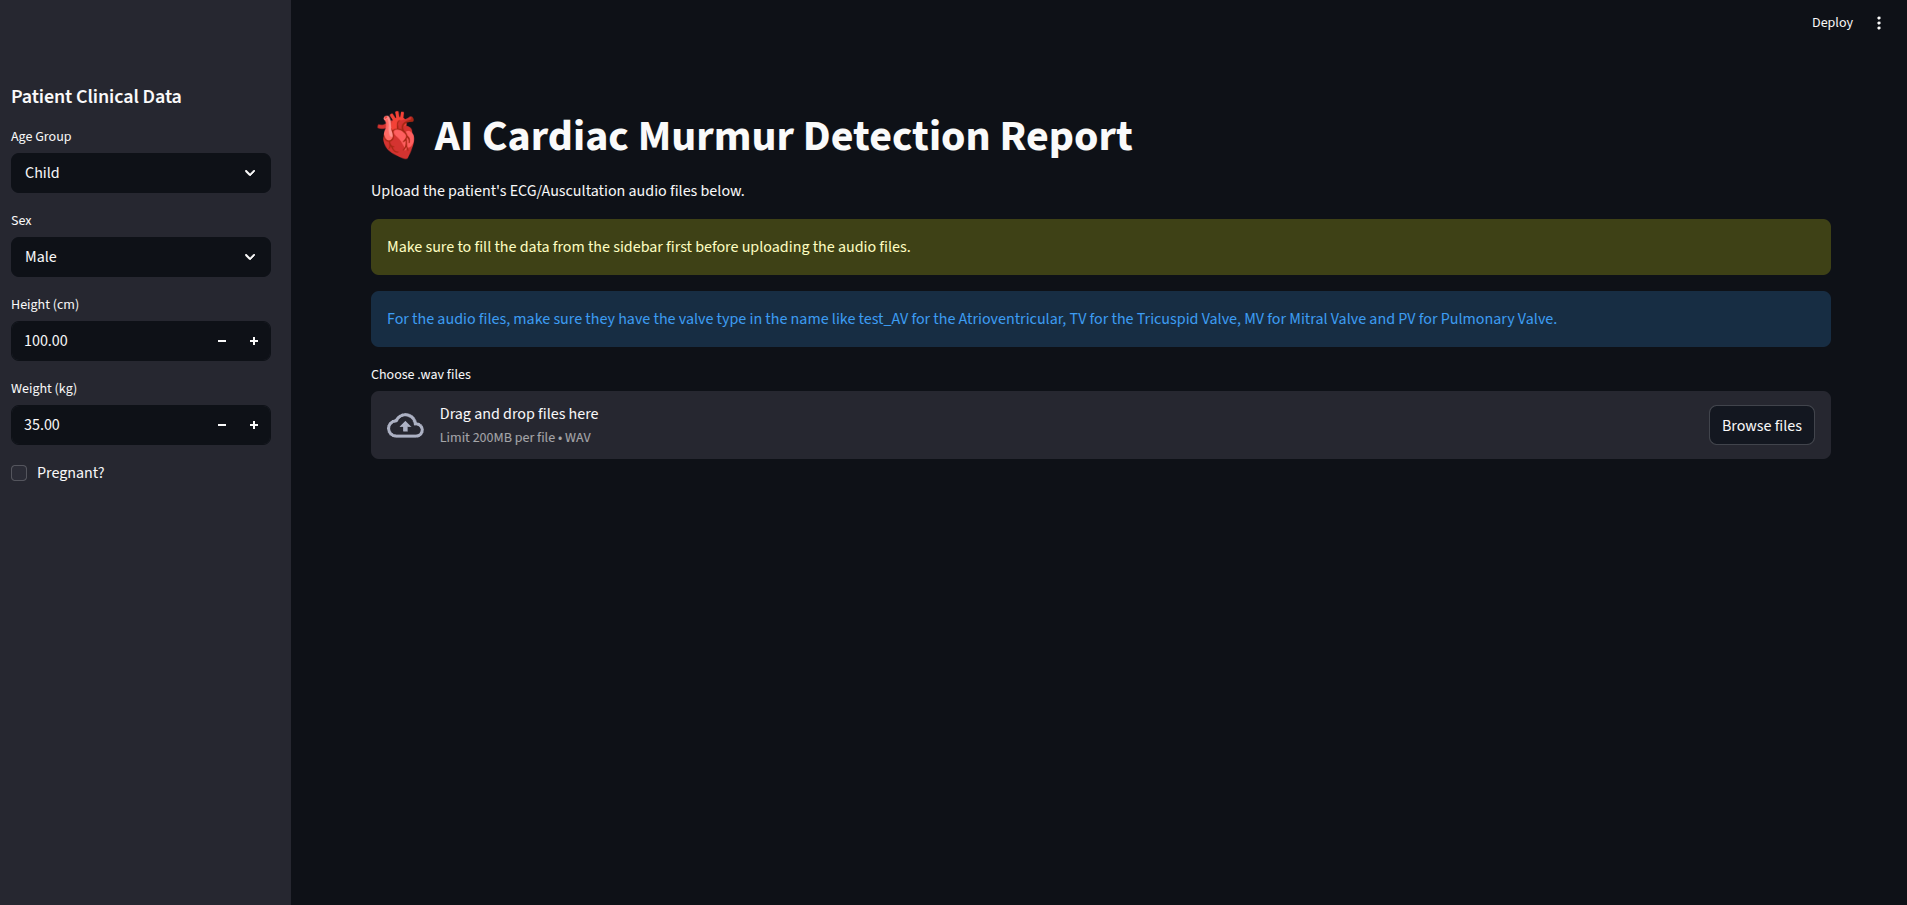
\includegraphics[width=1\textwidth]{streamlit_home.png}
    \caption{Left: Streamlit interface when opened.}
\end{figure}

Physicians can upload multiple audio files simultaneously. The system processes the audio, applies the mathematical scaling to clinical inputs, and generates a fully formatted PDF report detailing the AI's confidence levels and plotting the exact spectrogram windows that triggered anomalies. 

\begin{figure}[htbp]
    \centering
    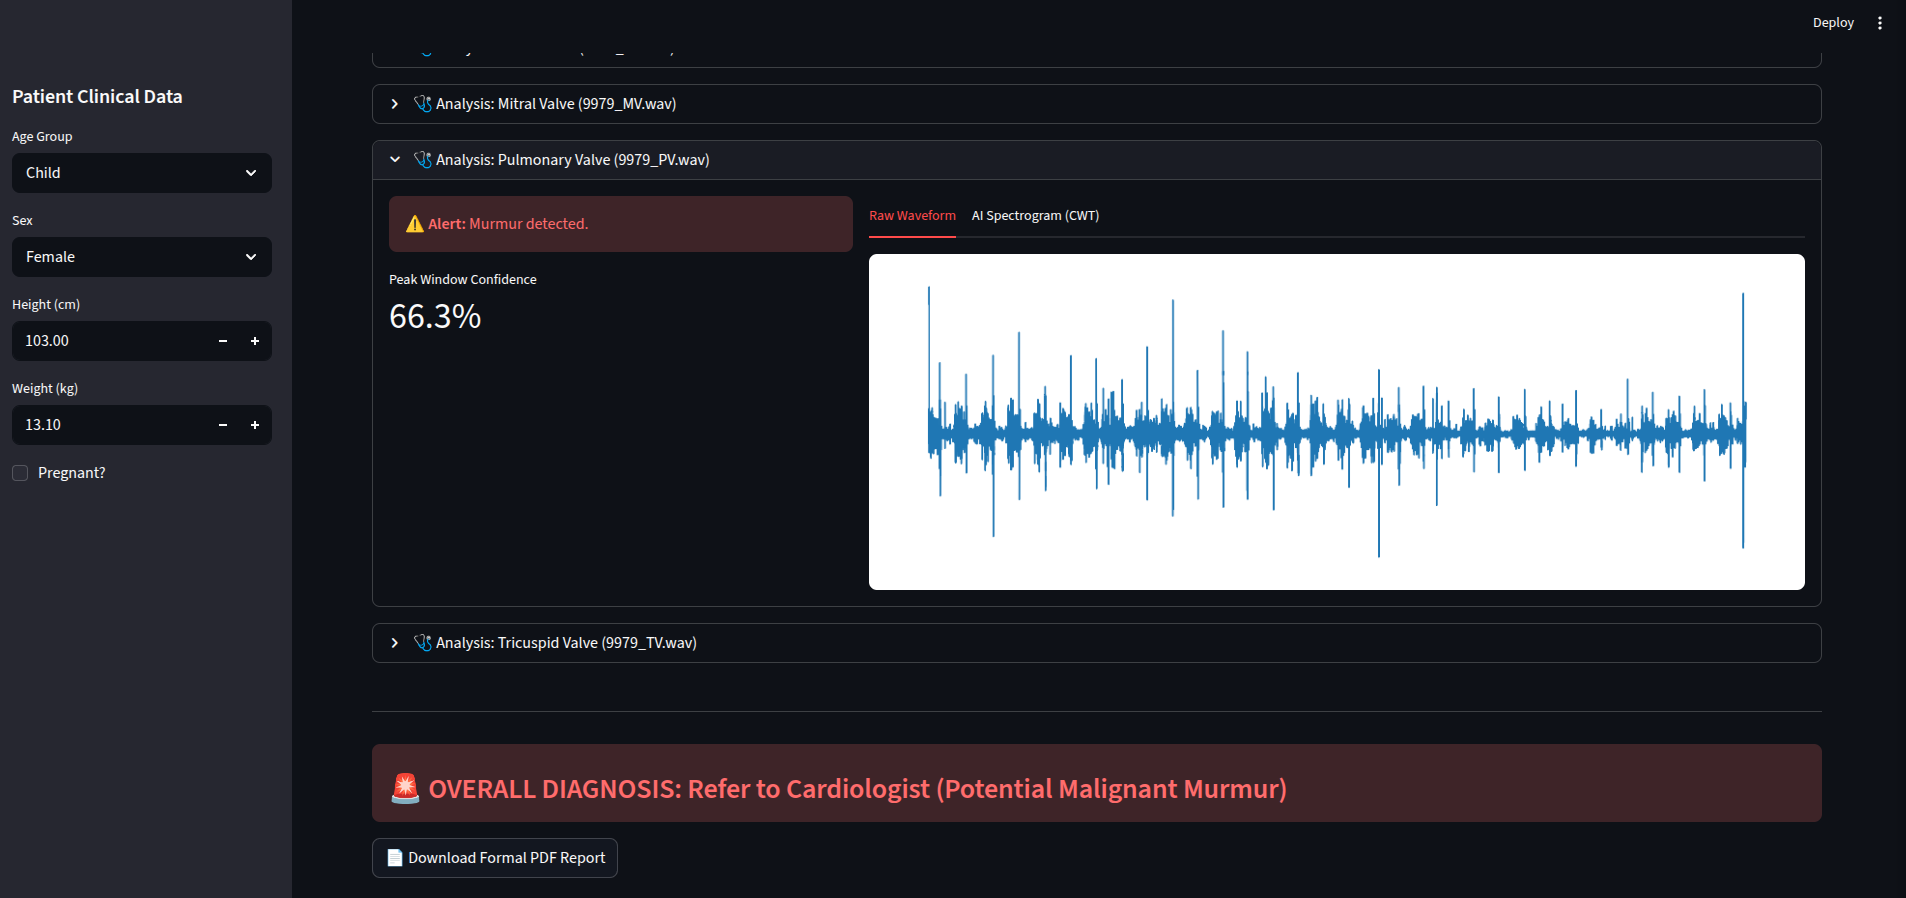
\includegraphics[width=1\textwidth]{streamlit_result.png}
    \caption{The model finds high chance of a malignant murmur.}
\end{figure}

% --- Section 8: Conclusions ---
\section{Conclusions}
This project successfully designed, trained, and deployed a leakage-free, multi-modal Deep Learning framework capable of detecting malignant heart murmurs with an accuracy approaching 70\% and an AUC of 0.76. 

By leveraging Continuous Wavelet Transforms, multi-modal context, and patient-level aggregation, the system overcomes the inherent noise of real-world auscultation. The resulting tool proves that artificial intelligence can effectively serve as a robust, objective pre-screening layer in primary care, catching anomalies that might otherwise be missed by the human ear.

\textbf{Future Work:}
Subsequent iterations should focus on targeted audio Data Augmentation (time-stretching and pitch-shifting) to further immunize the model against varying stethoscope hardware, and conducting a live clinical pilot to benchmark the AI directly against attending physicians in real time.

In this repo you can check out the code for this project in its entirety: \href{https://github.com/Starkiller747/cardiac_murmur}{Github Repo}

The streamlit application is also live on: \href{https://cardiacmurmur-unam.streamlit.app/}{Streamlit Live App}

\newpage

% This single command replaces the entire \begin{thebibliography} block
\printbibliography

\end{document}